%=======================================================================
%  CH 3 — NUMERICAL PROBLEMS & SOLUTIONS
%=======================================================================
\section*{\color{acc}Ch 3 --- Classification --- Numerical Problems \& Solutions}
\vspace{-4pt}{\color{acc}\rule{\textwidth}{1.1pt}}\vspace{4pt}

{\color{sub}\footnotesize 6 distinct methods $\cdot$ 12 PYQ instances solved $\cdot$
every answer independently recomputed. Decision-tree and Naive-Bayes figures cross-checked against
Han \& Kamber 3rd ed Examples 8.1--8.4, which use the same dataset the IOE papers copy.}

\lead{Methods}
\begin{itemize}
  \item \textbf{M1} Decision tree by information gain (ID3) \hfill \yr{79 Bh, 78 Bh, 76 Ch}
  \item \textbf{M2} Gini index \hfill \yr{75 Ch, 71 Ch}
  \item \textbf{M3} Naive Bayes classification \hfill \yr{72 Ch, 79 Bh}
  \item \textbf{M4} $k$-Nearest Neighbour \hfill \yr{80 Bh}
  \item \textbf{M5} Confusion matrix metrics \hfill \mk{8 papers}
  \item \textbf{M6} ANN gradients (backpropagation) \hfill \yr{76 Ch}
\end{itemize}

\hr

%=======================================================================
\T{M1. Decision tree by information gain (ID3)}

\lead{Method}
\begin{enumerate}
  \item Compute $Info(D) = -\sum p_i \log_2 p_i$ for the whole set.
  \item For each attribute $A$: split $D$, compute
        $Info_A(D)=\sum \frac{|D_j|}{|D|}Info(D_j)$, then $Gain(A)=Info(D)-Info_A(D)$.
  \item \textbf{Highest gain wins} $\rightarrow$ becomes the node's test.
  \item Recurse on each branch. Stop when a branch is \textbf{pure} ($Info = 0$).
\end{enumerate}
\begin{itemize}
  \item \mk{Time-savers}: a pure partition contributes $0$; a 50/50 partition contributes exactly $1$;
        two partitions with the same class ratio have the same $Info$, so compute once.
  \item $\log_2 x = \ln x / \ln 2$. Keep 4 decimals until the end.
\end{itemize}

\creamq{Problem 1.1}{\m{10}}
\begin{asked}{2079 Bhadra \textperiodcentered{} Q3 \textperiodcentered{} [10]}
Draw decision tree for the given data using ID3 algorithm.
\par\vspace{2pt}
\begin{tabularx}{0.80\textwidth}{@{}L{2.3cm}L{1.8cm}L{1.7cm}L{2.5cm}X@{}}
\toprule
\hrow \thead{Age} & \thead{Income} & \thead{Student} & \thead{Credit\_Rating} & \thead{Buy's\_Computer} \\
Youth       & High   & No  & Fair      & No  \\
Youth       & High   & No  & Excellent & No  \\
Middle\_Aged & High   & No  & Fair      & Yes \\
Senior      & Medium & No  & Fair      & Yes \\
Senior      & Low    & Yes & Fair      & Yes \\
Senior      & Low    & Yes & Excellent & No  \\
Middle\_Aged & Low    & Yes & Excellent & Yes \\
Youth       & Medium & No  & Fair      & No  \\
Youth       & Low    & Yes & Fair      & Yes \\
Senior      & Medium & Yes & Fair      & Yes \\
Youth       & Medium & Yes & Excellent & Yes \\
Middle\_Aged & Medium & No  & Excellent & Yes \\
Middle\_Aged & High   & Yes & Fair      & Yes \\
Senior      & Medium & No  & Excellent & No  \\
\bottomrule
\end{tabularx}
\end{asked}

\lead{Given} 14 tuples. Class counts: \textbf{Yes $=$ 9}, \textbf{No $=$ 5}.

\lead{Step 1: entropy of the whole set}
\[ Info(D) = -\tfrac{9}{14}\log_2\tfrac{9}{14} - \tfrac{5}{14}\log_2\tfrac{5}{14}
   = 0.4098 + 0.5305 = \mathbf{0.940} \]

\lead{Step 2: gain of each attribute}
\begin{tabularx}{\textwidth}{@{}L{2.4cm}L{4.3cm}XL{1.9cm}@{}}
\toprule
\hrow \thead{Attribute} & \thead{Partition (Yes, No)} & \thead{$Info_A(D)$} & \thead{Gain} \\
\textbf{Age} & Youth (2,3) $\cdot$ Middle\_Aged (4,0) $\cdot$ Senior (3,2) &
$\tfrac{5}{14}(0.971)+\tfrac{4}{14}(0)+\tfrac{5}{14}(0.971)=0.694$ & $\mathbf{0.246}$ \\
Income & High (2,2) $\cdot$ Medium (4,2) $\cdot$ Low (3,1) &
$\tfrac{4}{14}(1.0)+\tfrac{6}{14}(0.918)+\tfrac{4}{14}(0.811)=0.911$ & 0.029 \\
Student & Yes (6,1) $\cdot$ No (3,4) &
$\tfrac{7}{14}(0.592)+\tfrac{7}{14}(0.985)=0.788$ & 0.151 \\
Credit\_Rating & Fair (6,2) $\cdot$ Excellent (3,3) &
$\tfrac{8}{14}(0.811)+\tfrac{6}{14}(1.0)=0.892$ & 0.048 \\
\bottomrule
\end{tabularx}

\begin{itemize}
  \item \mk{Age has the highest gain $\rightarrow$ Age is the root.}
  \item Note Middle\_Aged is $(4,0)$: \textbf{pure}, so that branch is immediately a leaf ``Yes''.
        That purity is what makes Age win.
\end{itemize}

\lead{Step 3: recurse on the Youth branch} (5 tuples: 2 Yes, 3 No, $Info = 0.971$)
\begin{itemize}
  \item Student $=$ Yes $\rightarrow$ (2 Yes, 0 No) \quad Student $=$ No $\rightarrow$ (0 Yes, 3 No)
  \item Both pure $\rightarrow$ $Info_{Student}=0$ $\rightarrow$ $Gain = 0.971$, the maximum possible.
  \item \textbf{Student} is the test under Youth.
\end{itemize}

\lead{Step 4: recurse on the Senior branch} (5 tuples: 3 Yes, 2 No, $Info = 0.971$)
\begin{itemize}
  \item Credit $=$ Fair $\rightarrow$ (3 Yes, 0 No) \quad Credit $=$ Excellent $\rightarrow$ (0 Yes, 2 No)
  \item Both pure $\rightarrow$ $Gain = 0.971$. \textbf{Credit\_Rating} is the test under Senior.
\end{itemize}

\sbsr{0.46}{%
\lead{Final tree}
\begin{itemize}
  \item \textbf{Age?}
  \begin{itemize}
    \item \emph{Youth} $\rightarrow$ \textbf{Student?}
    \begin{itemize}
      \item no $\rightarrow$ \textbf{No}
      \item yes $\rightarrow$ \textbf{Yes}
    \end{itemize}
    \item \emph{Middle\_Aged} $\rightarrow$ \textbf{Yes}
    \item \emph{Senior} $\rightarrow$ \textbf{Credit\_Rating?}
    \begin{itemize}
      \item fair $\rightarrow$ \textbf{Yes}
      \item excellent $\rightarrow$ \textbf{No}
    \end{itemize}
  \end{itemize}
  \item Tree has \textbf{5 leaves}, depth 2, and classifies all 14 training tuples correctly.
\end{itemize}}{%
\figT{dt_example}
{\color{sub}\footnotesize The same tree as printed in Han \& Kamber 3rd ed, Fig 8.2. Our
independently computed gains match their Example 8.1 exactly.}}

\creamq{Problem 1.2}{\m{8}}
\begin{asked}{2078 Bhadra \textperiodcentered{} Q4 \textperiodcentered{} [8]}
Construct a decision tree for the following data set using information gain.

Predict the class label for a data point with values $<$Female, 2, standard, high$>$
\par\vspace{2pt}
\begin{tabularx}{0.86\textwidth}{@{}L{1.7cm}L{2.6cm}L{2.2cm}L{2.4cm}X@{}}
\toprule
\hrow \thead{Gender} & \thead{Car ownership} & \thead{Travel cost} & \thead{Income level} & \thead{Transport mode} \\
Male   & 0 & Cheap     & Low    & Bus   \\
Male   & 1 & Cheap     & Medium & Bus   \\
Female & 0 & Cheap     & Low    & Bus   \\
Male   & 1 & Cheap     & Medium & Bus   \\
Female & 1 & Expensive & High   & Car   \\
Male   & 2 & Expensive & Medium & Car   \\
Female & 2 & Expensive & High   & Car   \\
Female & 1 & Cheap     & Medium & Train \\
Male   & 0 & Standard  & Medium & Train \\
Female & 1 & Standard  & Medium & Train \\
\bottomrule
\end{tabularx}
\end{asked}

\lead{Given} Classes: Bus $=$ 4, Car $=$ 3, Train $=$ 3. \quad $n = 10$.
\[ Info(D) = -\tfrac{4}{10}\log_2\tfrac{4}{10} - \tfrac{3}{10}\log_2\tfrac{3}{10}
   - \tfrac{3}{10}\log_2\tfrac{3}{10} = 0.5288+0.5211+0.5211 = \mathbf{1.571} \]

\lead{Travel cost} \ Cheap (4 Bus, 0 Car, 1 Train) $\cdot$ Expensive (0,3,0) $\cdot$ Standard (0,0,2)
\begin{itemize}
  \item $Info(\text{Cheap}) = -\tfrac{4}{5}\log_2\tfrac{4}{5}-\tfrac{1}{5}\log_2\tfrac{1}{5} = 0.722$
  \item Expensive and Standard are both \textbf{pure} $\rightarrow$ $Info = 0$
  \item $Info_{TravelCost}(D) = \tfrac{5}{10}(0.722) + \tfrac{3}{10}(0) + \tfrac{2}{10}(0) = 0.361$
  \item $Gain = 1.571 - 0.361 = \mathbf{1.210}$
\end{itemize}
\begin{itemize}
  \item Every other attribute scores far lower (Gender $0.125$, Car ownership $0.534$,
        Income level $0.971$), so \mk{Travel cost is the root} --- two of its three branches are pure.
  \item Only the \emph{Cheap} branch needs splitting: 5 tuples (4 Bus, 1 Train). Splitting it on
        \textbf{Gender} gives Male (3 Bus, 0 Train) and Female (1 Bus, 1 Train); splitting on
        \textbf{Car ownership} gives 0 (2 Bus), 1 (2 Bus, 1 Train). Neither is perfect;
        Gender has the higher gain, then Car ownership finishes the Female sub-branch.
\end{itemize}

\lead{Prediction for $<$Female, 2, standard, high$>$}
\begin{itemize}
  \item Travel cost $=$ \textbf{standard} $\rightarrow$ that branch is \textbf{pure Train}.
  \item \mk{No further tests are needed.} \quad \textbf{Answer: Train.}
\end{itemize}

\hr

%=======================================================================
\T{M2. Gini index}

\lead{Method}
\[ Gini(D) = 1-\sum_i p_i^2 \qquad
   Gini_A(D) = \tfrac{|D_1|}{|D|}Gini(D_1)+\tfrac{|D_2|}{|D|}Gini(D_2) \qquad
   \Delta Gini = Gini(D)-Gini_A(D) \]
\begin{itemize}
  \item \mk{Gini uses BINARY splits only.} For an attribute with $v$ values you must try all
        $2^{v-1}-1$ ways of splitting the values into 2 subsets and keep the best.
  \item Pick the largest $\Delta Gini$ (equivalently the smallest $Gini_A$).
\end{itemize}

\creamq{Worked example (same 14-tuple dataset)}{\m{6}}
\begin{asked}{2075 Chaitra \textperiodcentered{} Q3 \textperiodcentered{} [6+4]}
Define Decision Tree Classifier with Gini-Index with suitable example. How can you handle
overfitting in Decision Tree?
\end{asked}
\begin{asked}{2071 Chaitra \textperiodcentered{} Q3 \textperiodcentered{} [10]}
What is a decision tree? Explain Gini Index with suitable example.
\end{asked}
{\color{sub}\footnotesize Neither paper prints a dataset --- the ``suitable example'' is yours to
supply. The 14-tuple \emph{buys\_computer} set below is the safe one to reuse. \added}

\begin{itemize}
  \item $Gini(D) = 1 - \left(\tfrac{9}{14}\right)^2 - \left(\tfrac{5}{14}\right)^2
        = 1 - 0.4133 - 0.1276 = \mathbf{0.459}$
  \item Split \textbf{Income} as \{low, medium\} vs \{high\}:
  \begin{itemize}
    \item $D_1$ $=$ 10 tuples (7 Yes, 3 No): $Gini = 1-(0.7)^2-(0.3)^2 = 0.420$
    \item $D_2$ $=$ 4 tuples (2 Yes, 2 No): $Gini = 1-(0.5)^2-(0.5)^2 = 0.500$
    \item $Gini_{Income}(D) = \tfrac{10}{14}(0.420)+\tfrac{4}{14}(0.500) = 0.300+0.143 = 0.443$
    \item $\Delta Gini = 0.459-0.443 = \mathbf{0.016}$
  \end{itemize}
  \item Split \textbf{Age} as \{youth, senior\} vs \{middle\_aged\}:
  \begin{itemize}
    \item $D_1$ $=$ 10 tuples (5 Yes, 5 No): $Gini = 0.500$
    \item $D_2$ $=$ 4 tuples (4 Yes, 0 No): $Gini = \mathbf{0}$ (pure)
    \item $Gini_{Age}(D) = \tfrac{10}{14}(0.500)+\tfrac{4}{14}(0) = 0.357$
    \item $\Delta Gini = 0.459-0.357 = \mathbf{0.102}$ \mk{$\rightarrow$ best, so Age is chosen}
  \end{itemize}
  \item Same winner as information gain, which is the usual (not guaranteed) outcome.
\end{itemize}

\hr

%=======================================================================
\T{M3. Naive Bayes classification}

\lead{Method}
\begin{enumerate}
  \item Priors: $P(C_i) = |C_{i,D}|/|D|$.
  \item For each attribute value in $X$: $P(x_k|C_i)$ from counts within class $C_i$.
  \item $P(X|C_i) = \prod_k P(x_k|C_i)$.
  \item Compare $P(X|C_i)P(C_i)$ across classes; \textbf{largest wins}.
\end{enumerate}
\begin{itemize}
  \item \mk{Never divide by $P(X)$} --- it is identical for every class and cancels.
  \item Any zero count $\rightarrow$ apply \textbf{Laplacian correction} $\frac{n_k+1}{|C_{i,D}|+k}$.
  \item Lay the work out as a small table of conditional probabilities; it earns method marks even
        if arithmetic slips.
\end{itemize}

\creamq{Problem 3.1}{\m{10}}
\begin{asked}{2072 Chaitra \textperiodcentered{} Q3 \textperiodcentered{} [10]}
Predict Class label using naive Bayesian classifier for $X =$ (age $=$ youth, income $=$
medium, student $=$ yes, credit-rating $=$ fair) using the following data set.
\par\vspace{2pt}
\begin{tabularx}{0.86\textwidth}{@{}L{0.9cm}L{2.3cm}L{1.7cm}L{1.6cm}L{2.4cm}X@{}}
\toprule
\hrow \thead{RID} & \thead{Age} & \thead{Income} & \thead{Student} & \thead{Credit-rating} & \thead{Class Buy computer} \\
1  & Youth       & High   & No  & Fair      & No  \\
2  & Youth       & High   & No  & Excellent & No  \\
3  & Middle-age & High   & No  & Fair      & Yes \\
4  & Senior      & Medium & No  & Fair      & Yes \\
5  & Senior      & Low    & Yes & Fair      & Yes \\
6  & Senior      & Low    & Yes & Excellent & No  \\
7  & Middle-age & Low    & Yes & Excellent & Yes \\
8  & Youth       & Medium & No  & Fair      & No  \\
9  & Youth       & Low    & Yes & Fair      & Yes \\
10 & Senior      & Medium & Yes & Fair      & Yes \\
11 & Youth       & Medium & Yes & Excellent & Yes \\
12 & Middle-age & Medium & No  & Excellent & Yes \\
13 & Middle-age & High   & Yes & Fair      & Yes \\
14 & Senior      & Medium & No  & Excellent & No  \\
\bottomrule
\end{tabularx}
\end{asked}

\lead{Given} 14 tuples. $P(\text{Yes}) = 9/14 = 0.643$, \ $P(\text{No}) = 5/14 = 0.357$.

\sbs{%
\lead{Conditional probabilities}
\begin{tabularx}{\linewidth}{@{}L{3.4cm}XX@{}}
\toprule
\hrow & \thead{$|$Yes} & \thead{$|$No} \\
$P(\text{age}=\text{youth})$   & $2/9=0.222$ & $3/5=0.600$ \\
$P(\text{income}=\text{med})$  & $4/9=0.444$ & $2/5=0.400$ \\
$P(\text{student}=\text{yes})$ & $6/9=0.667$ & $1/5=0.200$ \\
$P(\text{credit}=\text{fair})$ & $6/9=0.667$ & $2/5=0.400$ \\
\bottomrule
\end{tabularx}}{%
\lead{Combine}
\begin{itemize}
  \item $P(X|\text{Yes}) = 0.222\times0.444\times0.667\times0.667 = \mathbf{0.0439}$
  \item $P(X|\text{No}) = 0.600\times0.400\times0.200\times0.400 = \mathbf{0.0192}$
  \item $P(X|\text{Yes})P(\text{Yes}) = 0.0439\times0.643 = \mathbf{0.028}$
  \item $P(X|\text{No})P(\text{No}) = 0.0192\times0.357 = \mathbf{0.007}$
\end{itemize}}

\lead{Final answer} $0.028 > 0.007$ $\rightarrow$ \mk{buys\_computer $=$ \textbf{Yes}}.
\begin{itemize}
  \item Matches Han \& Kamber 3rd ed Example 8.4.
\end{itemize}

\creamq{Problem 3.2}{\m{6}}
\begin{asked}{2079 Bhadra \textperiodcentered{} Q4 \textperiodcentered{} [6]}
Suppose you have a test record ``$X =$ (Home Owner $=$ No, Material Status $=$ Married,
Income $=$ \$120K)''. Your job is to classify this record using Naive Bayesian Classification.
Use the following table for your calculations.
\par\vspace{2pt}
\begin{tabularx}{0.80\textwidth}{@{}L{0.9cm}L{2.3cm}L{2.6cm}L{2.6cm}X@{}}
\toprule
\hrow \thead{Tid} & \thead{Home Owner} & \thead{Marital Status} & \thead{Annual Income} & \thead{Defaulted Borrower} \\
1  & Yes & Single   & 125K & No  \\
2  & No  & Married  & 100K & No  \\
3  & No  & Single   & 70K  & No  \\
4  & Yes & Married  & 120K & No  \\
5  & No  & Divorced & 95K  & Yes \\
6  & No  & Married  & 60K  & No  \\
7  & Yes & Divorced & 220K & No  \\
8  & No  & Single   & 85K  & Yes \\
9  & No  & Married  & 75K  & No  \\
10 & No  & Single   & 90K  & Yes \\
\bottomrule
\end{tabularx}
\end{asked}

\lead{Given} Defaulted: \textbf{No $=$ 7}, \textbf{Yes $=$ 3}. $P(\text{No})=0.7$, $P(\text{Yes})=0.3$.

\lead{Step 1: categorical attributes}
\begin{itemize}
  \item $P(\text{HO}=\text{No}\,|\,\text{No}) = 4/7 = 0.571$ \qquad
        $P(\text{HO}=\text{No}\,|\,\text{Yes}) = 3/3 = 1.0$
  \item $P(\text{Married}\,|\,\text{No}) = 4/7 = 0.571$ \qquad
        $P(\text{Married}\,|\,\text{Yes}) = \mathbf{0/3 = 0}$ \mk{$\leftarrow$ zero!}
\end{itemize}
\begin{itemize}
  \item Apply \textbf{Laplacian correction} (Marital Status has $k=3$ values):
        $P(\text{Married}|\text{Yes}) = \frac{0+1}{3+3} = 0.167$;
        and $P(\text{HO}=\text{No}|\text{Yes}) = \frac{3+1}{3+2} = 0.8$.
\end{itemize}

\lead{Step 2: continuous attribute (Income), Gaussian}
\[ g(x,\mu,\sigma) = \frac{1}{\sqrt{2\pi}\,\sigma}\,e^{-\frac{(x-\mu)^2}{2\sigma^2}} \]
\begin{itemize}
  \item Class \textbf{No}: incomes 125, 100, 70, 120, 60, 220, 75 $\rightarrow$
        $\mu = 110$, $\sigma = 54.54$
        \[ g(120) = \tfrac{1}{\sqrt{2\pi}(54.54)}e^{-\frac{(10)^2}{2(2975)}} = 0.00719 \]
  \item Class \textbf{Yes}: incomes 95, 85, 90 $\rightarrow$ $\mu = 90$, $\sigma = 5$
        \[ g(120) = \tfrac{1}{\sqrt{2\pi}(5)}e^{-\frac{(30)^2}{2(25)}} = 0.0798\,e^{-18}
           \approx 1.2\times10^{-9} \]
  \item \mk{The Yes class has a tiny spread ($\sigma=5$) around \$90K, so \$120K is 6 standard
        deviations out} --- effectively impossible under that model.
\end{itemize}

\lead{Step 3: combine}
\begin{itemize}
  \item $P(X|\text{No})P(\text{No}) = 0.571\times0.571\times0.00719\times0.7 = \mathbf{1.64\times10^{-3}}$
  \item $P(X|\text{Yes})P(\text{Yes}) = 0.8\times0.167\times1.2\times10^{-9}\times0.3
        \approx \mathbf{4.8\times10^{-11}}$
\end{itemize}

\lead{Final answer} \mk{Defaulted Borrower $=$ \textbf{No}} (larger by roughly $10^{7}$).

\hr

%=======================================================================
\T{M4. $k$-Nearest Neighbour}

\lead{Method}
\begin{enumerate}
  \item Compute the Euclidean distance from the query to \textbf{every} training tuple.
  \item Sort ascending, take the $k$ smallest.
  \item \textbf{Majority class} among those $k$ is the prediction.
\end{enumerate}
\begin{itemize}
  \item \mk{Show the full distance table} --- that is where the marks are, not the final label.
  \item You may compare squared distances to save time, but write the roots in the final table.
\end{itemize}

\creamq{Problem 4.1}{\m{6}}
\begin{asked}{2080 Bhadra \textperiodcentered{} Q2 (b) \textperiodcentered{} [3+6]}
When do we use classifier? You have the following information about the flower. Your job is
to classify the given flower with SepalLength $=$ 7, SepalWidth $=$ 3.2, PetalLength $=$ 4.7,
and PetalWidth $=$ 1.4. Use KNN algorithm for $K = 3$ with Euclidean distance matrix.
\par\vspace{2pt}
\begin{tabularx}{0.86\textwidth}{@{}L{0.9cm}L{2.3cm}L{2.1cm}L{2.2cm}L{2.2cm}X@{}}
\toprule
\hrow \thead{Id} & \thead{Sepal\_Lenth} & \thead{Spal\_Width} & \thead{Petal\_Lenth} & \thead{Petal\_Width} & \thead{Labal} \\
1 & 5.1 & 3.5 & 1.4 & 0.2 & setosa \\
2 & 4.9 & 3   & 1.4 & 0.2 & setosa \\
3 & 4.7 & 3.2 & 1.3 & 0.2 & setosa \\
4 & 6   & 2.2 & 4   & 1   & versicolor \\
5 & 6.1 & 2.9 & 4.7 & 1.4 & versicolor \\
6 & 5.6 & 2.9 & 3.6 & 1.3 & versicolor \\
7 & 6.7 & 3.1 & 4.4 & 1.4 & versicolor \\
\bottomrule
\end{tabularx}
\vspace{2pt}
{\color{sub}Column names are the paper's own spellings.}
\end{asked}

\begin{tabularx}{\textwidth}{@{}L{0.9cm}L{4.6cm}XL{1.5cm}L{2.1cm}@{}}
\toprule
\hrow \thead{Id} & \thead{Tuple} & \thead{Squared differences} & \thead{$d$} & \thead{Label} \\
1 & (5.1, 3.5, 1.4, 0.2) & $3.61+0.09+10.89+1.44=16.03$ & 4.004 & setosa \\
2 & (4.9, 3.0, 1.4, 0.2) & $4.41+0.04+10.89+1.44=16.78$ & 4.096 & setosa \\
3 & (4.7, 3.2, 1.3, 0.2) & $5.29+0+11.56+1.44=18.29$ & 4.277 & setosa \\
4 & (6.0, 2.2, 4.0, 1.0) & $1+1+0.49+0.16=2.65$ & \textbf{1.628} & versicolor \\
5 & (6.1, 2.9, 4.7, 1.4) & $0.81+0.09+0+0=0.90$ & \textbf{0.949} & versicolor \\
6 & (5.6, 2.9, 3.6, 1.3) & $1.96+0.09+1.21+0.01=3.27$ & 1.808 & versicolor \\
7 & (6.7, 3.1, 4.4, 1.4) & $0.09+0.01+0.09+0=0.19$ & \textbf{0.436} & versicolor \\
\bottomrule
\end{tabularx}

\lead{Step: pick the 3 nearest}
\begin{itemize}
  \item Sorted: \ $d_7 = 0.436$ \ $<$ \ $d_5 = 0.949$ \ $<$ \ $d_4 = 1.628$ \ $<$ \ $d_6 = 1.808$
        \ $<$ \ $d_1 = 4.004 \dots$
  \item The 3 nearest are \textbf{Id 7, Id 5, Id 4} $\rightarrow$ versicolor, versicolor, versicolor.
\end{itemize}

\lead{Final answer} \mk{\textbf{versicolor}} (unanimous, 3 of 3).
\begin{itemize}
  \item Note all 3 setosa tuples sit at distance $>4$: they have tiny petals, so they are nowhere
        near the query. The vote was never in doubt.
\end{itemize}

\hr

%=======================================================================
\T{M5. Confusion matrix metrics \mk{(8 papers --- highest-yield numerical in the syllabus)}}

\begin{center}\fbox{\begin{minipage}{0.95\textwidth}\small
\mk{DO THIS FIRST, EVERY TIME.} Copy the row and column headings onto your answer sheet and mark
which axis is \textbf{actual}. The IOE papers \textbf{flip the orientation between years}. \\
Proof: \yr{75 Ash} and \yr{72 Ch} print the \emph{identical} four numbers 21, 6, 7, 41 --- but
75 Ash has actual on the rows and 72 Ch has predicted on the rows. The result is that
\textbf{sensitivity and precision swap places} (0.778 / 0.750 becomes 0.750 / 0.778).
Same numbers, different answers. \added
\end{minipage}}\end{center}

\lead{Method}
\begin{itemize}
  \item Identify $TP$, $FN$, $FP$, $TN$ from the orientation. Then
        $P = TP+FN$ (all actual positives), $N = FP+TN$ (all actual negatives).
  \item Accuracy $=\frac{TP+TN}{P+N}$ \quad Error $=1-$accuracy
  \item Sensitivity $=$ recall $=$ TPR $=\frac{TP}{P}$ \quad Specificity $=$ TNR $=\frac{TN}{N}$
  \item FPR $=$ false alarm rate $=\frac{FP}{N} = 1-$specificity \quad
        Precision $=\frac{TP}{TP+FP}$
\end{itemize}

\creamq{Problem 5.1}{\m{5}}
\begin{asked}{2074 Chaitra \textperiodcentered{} Q3 \textperiodcentered{} [2+3+5]}
Draw clear block diagram depicting different stages in classification. Explain the inverse
relation between precision and recall. Given the confusion matrix, determine accuracy,
sensitivity and precision of the classifier model.
\par\vspace{2pt}
\begin{tabularx}{0.60\textwidth}{@{}L{3.3cm}XX@{}}
\toprule
\hrow \thead{Actual $\backslash$ Predicted} & \thead{Positive} & \thead{Negative} \\
Positve  & 142 & 40  \\
Negative & 98  & 720 \\
\bottomrule
\end{tabularx}
\vspace{2pt}
{\color{sub}``Positve'' is the paper's own spelling.}
\end{asked}
\begin{itemize}
  \item $TP=142$, $FN=40$, $FP=98$, $TN=720$ $\rightarrow$ $P=182$, $N=818$, total $=1000$
  \item Accuracy $=\frac{142+720}{1000}= \mathbf{0.862}$
  \item Sensitivity $=\frac{142}{182}= \mathbf{0.780}$
  \item Precision $=\frac{142}{142+98}=\frac{142}{240}= \mathbf{0.592}$
  \item Specificity $=\frac{720}{818}= \mathbf{0.880}$
\end{itemize}

\creamq{Problem 5.2}{\m{4}}
\begin{asked}{2078 Bhadra \textperiodcentered{} Q6 \textperiodcentered{} [4]}
Calculate: Accuracy, TPR, FPR and Precision for the given confusion matrix for a classifier.
\par\vspace{2pt}
\begin{tabularx}{0.62\textwidth}{@{}L{2.6cm}L{1.9cm}XX@{}}
\toprule
\hrow & & \multicolumn{2}{@{}l}{\thead{Actual Class}} \\
\hrow & & \thead{Class 1} & \thead{Class 2} \\
\midrule
\textbf{Predicted Class} & Class 1 & 142 & 40 \\
 & Class 2 & 98 & 720 \\
\bottomrule
\end{tabularx}
\end{asked}
{\color{sub}\footnotesize \mk{Same four numbers as 5.1, but the rows are Predicted here.}}
\begin{itemize}
  \item Rows are predicted $\rightarrow$ $TP=142$, $FP=40$, $FN=98$, $TN=720$
  \item $P = 142+98 = 240$, \ $N = 40+720 = 760$
  \item Accuracy $=\frac{142+720}{1000}= \mathbf{0.862}$ \quad (unchanged --- the diagonal is the same)
  \item TPR $=\frac{142}{240}= \mathbf{0.592}$ \quad FPR $=\frac{40}{760}= \mathbf{0.053}$
  \item Precision $=\frac{142}{142+40}=\frac{142}{182}= \mathbf{0.780}$
  \item \mk{Compare with 5.1}: sensitivity and precision have exchanged values. This is the
        orientation trap, live.
\end{itemize}

\creamq{Problems 5.3 and 5.4}{\m{10}}
\begin{asked}{2075 Ashwin \textperiodcentered{} Q4 \textperiodcentered{} [10]}
The confusion matrix for a classifier is given as follows:
\par\vspace{2pt}
\begin{tabularx}{0.62\textwidth}{@{}L{2.6cm}L{1.9cm}XX@{}}
\toprule
\hrow & & \multicolumn{2}{@{}l}{\thead{Predicted Class}} \\
\hrow & & \thead{Class 1} & \thead{Class 2} \\
\midrule
\textbf{Actual Class} & Class 1 & 21 & 6 \\
 & Class 2 & 7 & 41 \\
\bottomrule
\end{tabularx}
\vspace{2pt}

Calculate: Accuracy, Sensitivity, Specificity and Precision.
\end{asked}
\begin{asked}{2072 Chaitra \textperiodcentered{} Q4 \textperiodcentered{} [10]}
The confusion matrix for a classifier is given as follows:
\par\vspace{2pt}
\begin{tabularx}{0.62\textwidth}{@{}L{2.6cm}L{1.9cm}XX@{}}
\toprule
\hrow & & \multicolumn{2}{@{}l}{\thead{actual class}} \\
\hrow & & \thead{class1} & \thead{class2} \\
\midrule
\textbf{predicted class} & class1 & 21 & 6 \\
 & class2 & 7 & 41 \\
\bottomrule
\end{tabularx}
\vspace{2pt}

Calculate a.~accuracy \quad b.~sensitivity \quad c.~specificity \quad d.~precision \quad e.~recall
\end{asked}
{\color{sub}\footnotesize \mk{Same four numbers, opposite orientation} --- that is the whole point
of solving them side by side.}

\sbs{%
\lead{75 Ash --- rows are Actual}
\begin{itemize}
  \item $TP=21$, $FN=6$, $FP=7$, $TN=41$; $P=27$, $N=48$, total $75$
  \item Accuracy $=\frac{62}{75}= \mathbf{0.827}$
  \item Sensitivity $=\frac{21}{27}= \mathbf{0.778}$
  \item Specificity $=\frac{41}{48}= \mathbf{0.854}$
  \item Precision $=\frac{21}{28}= \mathbf{0.750}$
\end{itemize}}{%
\lead{72 Ch --- rows are Predicted}
\begin{itemize}
  \item $TP=21$, $FP=6$, $FN=7$, $TN=41$; $P=28$, $N=47$, total $75$
  \item Accuracy $=\frac{62}{75}= \mathbf{0.827}$
  \item Sensitivity $=$ recall $=\frac{21}{28}= \mathbf{0.750}$
  \item Specificity $=\frac{41}{47}= \mathbf{0.872}$
  \item Precision $=\frac{21}{27}= \mathbf{0.778}$
\end{itemize}}

\creamq{Problem 5.5}{\m{10}}
\begin{asked}{2074 Ashwin \textperiodcentered{} Q4 \textperiodcentered{} [10]}
The confusion matrix for a classifier is given as follows:
\par\vspace{2pt}
\begin{tabularx}{0.62\textwidth}{@{}L{2.6cm}L{1.9cm}XX@{}}
\toprule
\hrow & & \multicolumn{2}{@{}l}{\thead{Predicted Class}} \\
\hrow & & \thead{Class 1} & \thead{Class 2} \\
\midrule
\textbf{Actual Class} & Class 1 & 25 & 9 \\
 & Class 2 & 4 & 31 \\
\bottomrule
\end{tabularx}
\vspace{2pt}

Calculate: \ a) Accuracy \quad b) Sensitivity \quad c) Specificity \quad d) Precision
\end{asked}
\begin{itemize}
  \item $TP=25$, $FN=9$, $FP=4$, $TN=31$; $P=34$, $N=35$, total $69$
  \item Accuracy $=\frac{56}{69}= \mathbf{0.812}$ \quad Sensitivity $=\frac{25}{34}= \mathbf{0.735}$
  \item Specificity $=\frac{31}{35}= \mathbf{0.886}$ \quad Precision $=\frac{25}{29}= \mathbf{0.862}$
\end{itemize}

\creamq{Problem 5.6}{\m{3+5}}
\begin{asked}{2080 Baishakh \textperiodcentered{} Q3 \textperiodcentered{} [3+5]}
In what cases you cannot use Accuracy for performance measure, give some examples. Assume
that you have the following confusion matrix. Calculate the Classification error, Sensitivity,
False alarm rate Specificity.
\par\vspace{2pt}
\begin{tabularx}{0.62\textwidth}{@{}L{2.6cm}L{1.9cm}XX@{}}
\toprule
\hrow & & \multicolumn{2}{@{}l}{\thead{Actual Values}} \\
\hrow & & \thead{True} & \thead{False} \\
\midrule
\textbf{Predicated Values} & True & 1050 & 250 \\
 & False & 150 & 950 \\
\bottomrule
\end{tabularx}
\end{asked}
\begin{itemize}
  \item $TP=1050$, $FP=250$, $FN=150$, $TN=950$; $P=1200$, $N=1200$, total $2400$
  \item Classification error $=\frac{250+150}{2400}= \mathbf{0.167}$
  \item Sensitivity $=\frac{1050}{1200}= \mathbf{0.875}$
  \item False alarm rate (FPR) $=\frac{250}{1200}= \mathbf{0.208}$
  \item Specificity $=\frac{950}{1200}= \mathbf{0.792}$ \quad (check: $0.208+0.792=1$ \checkmark)
\end{itemize}

\creamq{Problem 5.7}{\m{3+6}}
\begin{asked}{2073 Shrawan \textperiodcentered{} Q4 \textperiodcentered{} [1+3+6]}
Explain ROC. Using the following data, calculate TPR, FPR, precision for given confusion matrix.
\par\vspace{2pt}
\begin{tabularx}{0.40\textwidth}{@{}L{1.6cm}XX@{}}
\toprule
\hrow & \thead{A} & \thead{B} \\
A & 20 & 5  \\
B & 10 & 40 \\
\bottomrule
\end{tabularx}
\vspace{2pt}

Classify, A $=$ Yes, B $=$ No
\end{asked}
\begin{itemize}
  \item $TP=20$, $FN=5$, $FP=10$, $TN=40$; $P=25$, $N=50$
  \item TPR $=\frac{20}{25}= \mathbf{0.80}$ \quad FPR $=\frac{10}{50}= \mathbf{0.20}$
  \item Precision $=\frac{20}{30}= \mathbf{0.667}$
  \item The ROC point for this classifier is $(0.20,\ 0.80)$, comfortably above the diagonal.
\end{itemize}

\creamq{Problem 5.8}{\m{10}}
\begin{asked}{2070 Chaitra \textperiodcentered{} Q3 \textperiodcentered{} [10]}
An input sequence ``A A B B B A A A B B'' was used for classification. The Classifier `X'
predicted the sequences as: ``A A B B B A A A B B'' where as the Classifier `Y' predicted the
sequences as: ``A A A A B B A A A B''. Develop the corresponding confusion matrix for the
classifiers and find their corresponding.
\begin{enumerate}[label=\roman*), leftmargin=1.9em]
  \item Accuracy \quad ii) Precision \quad iii) True Positive Rate \quad iv) False Positive Rate
\end{enumerate}
\end{asked}

\lead{Step 1: tabulate Y position by position} (take A as the positive class)\par
\begin{tabularx}{\textwidth}{@{}L{1.6cm}XXXXXXXXXX@{}}
\toprule
\hrow Position & 1 & 2 & 3 & 4 & 5 & 6 & 7 & 8 & 9 & 10 \\
Actual & A & A & B & B & B & A & A & A & B & B \\
Y & A & A & A & A & B & B & A & A & A & B \\
Category & TP & TP & FP & FP & TN & FN & TP & TP & FP & TN \\
\bottomrule
\end{tabularx}

\sbs{%
\lead{Classifier X} (identical to actual)
\begin{itemize}
  \item $TP=5$, $TN=5$, $FP=0$, $FN=0$
  \item Accuracy $= \mathbf{1.0}$ \quad Precision $= \mathbf{1.0}$
  \item TPR $= \mathbf{1.0}$ \quad FPR $= \mathbf{0}$
  \item \mk{Perfect classifier} --- the ROC point is the top-left corner $(0,1)$.
\end{itemize}}{%
\lead{Classifier Y}
\begin{itemize}
  \item $TP=4$, $FN=1$, $FP=3$, $TN=2$; $P=5$, $N=5$ \ (total $10$ \checkmark)
  \item Accuracy $=\frac{4+2}{10}= \mathbf{0.60}$
  \item Precision $=\frac{4}{7}= \mathbf{0.571}$
  \item TPR $=\frac{4}{5}= \mathbf{0.80}$
  \item FPR $=\frac{3}{5}= \mathbf{0.60}$
\end{itemize}}
\begin{itemize}
  \item \mk{Reading}: Y has decent recall (0.80) but poor precision (0.571) --- it over-predicts A,
        firing 3 false alarms out of 5 actual Bs. Its ROC point $(0.60, 0.80)$ is only just above
        the diagonal, so it is barely better than guessing.
\end{itemize}

\hr

%=======================================================================
\T{M6. ANN gradients (backpropagation)}

\lead{Method}
\begin{itemize}
  \item Sigmoid and its derivative: $\sigma(z)=\frac{1}{1+e^{-z}}$, \quad
        $\sigma'(z)=\sigma(z)\big(1-\sigma(z)\big)$.
  \item Loss $E=\tfrac{1}{2}(o-t)^2$ \ $\rightarrow$ \ $\dfrac{\partial E}{\partial o} = (o-t)$.
  \item Apply the \textbf{chain rule} backwards from the loss to the weight in question.
\end{itemize}

\creamq{Problem 6.1}{\m{2+3+4}}
\begin{asked}{2076 Chaitra \textperiodcentered{} Q6 \textperiodcentered{} [2+3+4]}
Consider the multi-layer feed-forward neural network shown in the following figure. This
neural network has three inputs $x_1$, $x_2$ and $x_3$ connected to a hidden layer consisting
of two nodes $h_1$ and $h_2$. The weight of the edge connecting $x_i$ to $h_j$ is $w_{ji}$.
The two hidden nodes are connected to the output node $o$. The weight of the edge connecting
the hidden node $h_i$ to the output node $o$ is $u_i$. The activation functions at hidden and
output layers is set to sigmoid function defined as follows:
\[ \sigma(\theta) = \frac{1}{1+\exp(-\theta)} \]
Using the target output $t$, the squared error is used as the loss function at the output
node, and is defined as:
\[ E(o,t) = \tfrac{1}{2}(o-t)^2 \]
\begin{center}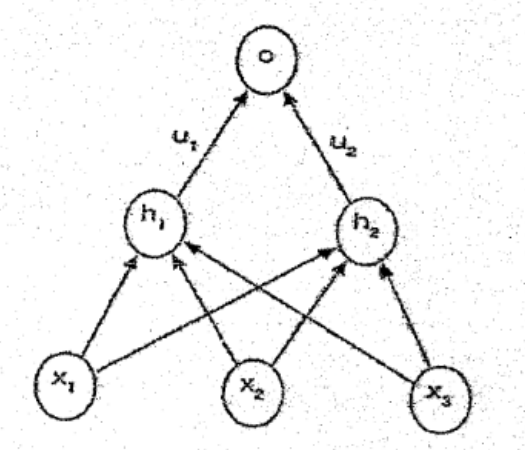
\includegraphics[width=0.44\textwidth]{figs/pyq_ann_76ch}\end{center}
\begin{enumerate}[label=\alph*), leftmargin=1.6em]
  \item Using the symbols given above, compute the activation at $h_1$.
  \item Compute the gradient of the loss with respect to the output $o$.
  \item Compute the gradient of the loss with respect to the weight $w_{12}$.
\end{enumerate}
\end{asked}

\lead{(a) Activation at $h_1$}
\[ h_1 = \sigma\big(w_{11}x_1 + w_{12}x_2 + w_{13}x_3\big)
       = \frac{1}{1+\exp\!\big(-(w_{11}x_1+w_{12}x_2+w_{13}x_3)\big)} \]

\lead{(b) Gradient of the loss w.r.t.\ the output $o$}
\[ E(o,t)=\tfrac{1}{2}(o-t)^2 \quad\Rightarrow\quad
   \frac{\partial E}{\partial o} = \mathbf{(o-t)} \]

\lead{(c) Gradient of the loss w.r.t.\ $w_{12}$}
\begin{itemize}
  \item $w_{12}$ is the weight from $x_2$ into $h_1$, so the chain runs
        $E \rightarrow o \rightarrow h_1 \rightarrow w_{12}$.
  \item Write $net_o = u_1h_1+u_2h_2$ and $net_{h_1}=w_{11}x_1+w_{12}x_2+w_{13}x_3$.
\end{itemize}
\[ \frac{\partial E}{\partial w_{12}}
   = \underbrace{\frac{\partial E}{\partial o}}_{(o-t)}\cdot
     \underbrace{\frac{\partial o}{\partial net_o}}_{o(1-o)}\cdot
     \underbrace{\frac{\partial net_o}{\partial h_1}}_{u_1}\cdot
     \underbrace{\frac{\partial h_1}{\partial net_{h_1}}}_{h_1(1-h_1)}\cdot
     \underbrace{\frac{\partial net_{h_1}}{\partial w_{12}}}_{x_2} \]
\[ \boxed{\ \frac{\partial E}{\partial w_{12}} = (o-t)\;o(1-o)\;u_1\;h_1(1-h_1)\;x_2\ } \]
\begin{itemize}
  \item \mk{Sanity checks}: the factor $x_2$ must appear (no input, no gradient); $u_1$ appears and
        $u_2$ does not, because $w_{12}$ only influences $o$ through $h_1$.
  \item Weight update: $w_{12} \leftarrow w_{12} - l\,\dfrac{\partial E}{\partial w_{12}}$.
\end{itemize}
